Aquest fotons creats en el plàstic de centelleig són detectats pels fotosensors. La col·laboració TRITIUM està investigant dos tipus de fotosensors diferents basats distintes propietats físiques, els tubs fotomultiplicadors (PMTs) i les matrius de fotomultiplicadors de silici (SiPMs).

El PMT, mostrat a la Figura \ref{subfig:PMT}, utilitza l'efecte fotoelèctric per transformar els fotons detectat en electrons. La matriu de SiPMs, mostrada a la Figura \ref{subfig:SiPM}, consisteix en diversos fotodíodes de avalancha operant en modo Geiger en paral·lel.

\begin{figure}[htpb]
\centering
    \begin{subfigure}[b]{0.4\textwidth}
    \centering
    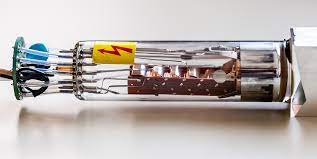
\includegraphics[width=\textwidth]{12Summary/3DesignPrinciples/32Tritium_detector/PMT.jpeg}  
    \caption{\label{subfig:PMT}}
    \end{subfigure}
    \hfill
    \begin{subfigure}[b]{0.4\textwidth}
    \centering
    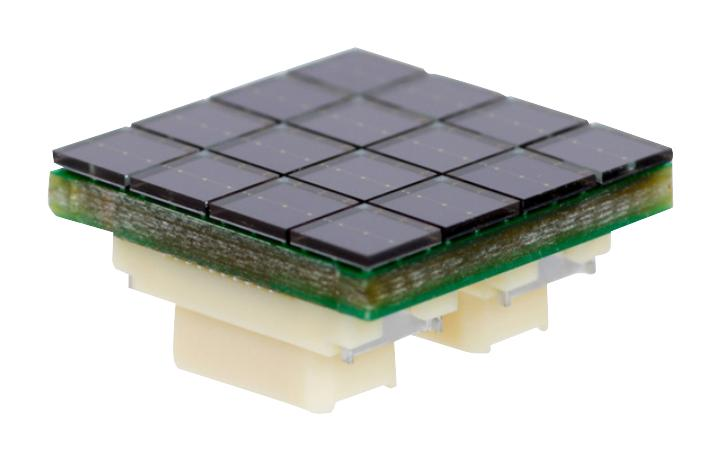
\includegraphics[width=\textwidth]{12Summary/3DesignPrinciples/32Tritium_detector/SiPM_Matrix.jpg}  
    \caption{\label{subfig:SiPM}}
    \end{subfigure}
 \caption{a) Tub fotomultiplicador. b) Matriu de fotomultiplicadors de silici.}
 \label{fig:Fotosensors}
\end{figure}

Els dos fotosensors posseeixen una àrea activa optimitzada per a la detecció de fotons, normalment en el rang energètic del visible. La probabilitat en què aquests produeixen un senyal com a resposta a la detecció de fotons ve donada per l'eficiència quàntica en el cas dels PMTs, Figura \ref{subfig:QEPMT} \cite{DataSheetPMTs}, i l'eficiència de fotodetecció per al cas dels SiPMs, Figura \ref{subfig:PDESiPM} \cite{DataSheetHammamatsu_1_SiPM_1375}.

\begin{figure}[htpb]
\centering
    \begin{subfigure}[b]{0.45\textwidth}
    \centering
    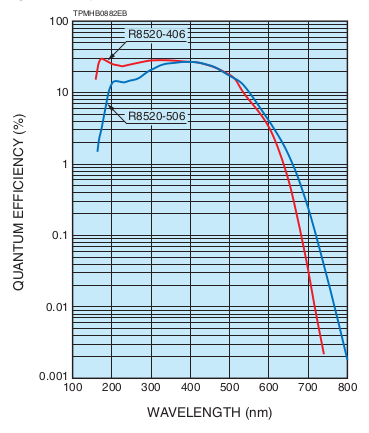
\includegraphics[width=\textwidth]{12Summary/3DesignPrinciples/32Tritium_detector/QuantumEfficiencyPMT.png}  
    \caption{\label{subfig:QEPMT}}
    \end{subfigure}
    \hfill
    \begin{subfigure}[b]{0.45\textwidth}
    \centering
    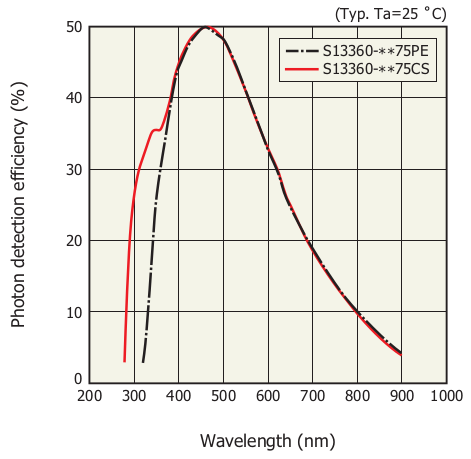
\includegraphics[width=\textwidth]{12Summary/3DesignPrinciples/32Tritium_detector/SiPMPDE.png}  
    \caption{\label{subfig:PDESiPM}}
    \end{subfigure}
 \caption{a) Eficiència quàntica del PMT model R8520-406 de Hamamatsu Photonics. b) Eficiència de fotodetecció del fotomultiplicador de silici model S13360-6075 de Hamamatsu Photonics.}
 \label{fig:EficienciaFotosensors}
\end{figure}

És important escollir el fotosensor adecuat per tal que l'espectre d'emissió del centellejador, Figura \ref{fig:EspectreEmisioPlasticsTRITIUM}, solape tant com siga possible amb l'eficiència de detecció del fotosensor, Figura \ref{fig:EficienciaFotosensors}, ja que l'eficiència del detector resultant dependrà del producte de tots dos.

Finalment els fotosensors emeten un senyal elèctric que porta informació de l'esdeveniment, el qual és amplificat per poder ser mesurat i analitzat. Aquest senyal és proporcional a la quantitat de fotons detectats i, per tant, a l'energia dipositada al centellejador per la partícula radioactiva. A partir de cert valor es perd aquesta linealitat i es produeix allò que s'anomena saturació.

Entre les principals diferències entre aquests dos fotosensors trobem que el SiPM no necessita alt voltatge per funcionar, té una major eficiència de detecció i és més robust mentre que el PMT presenta un soroll electrònic més baix. A mes, les propietats dels SiPMs varien fortament en funcio de la temperatura.

La col·laboració TRITIUM ha realitzat una caracterització detallada dels SiPMs obtenint amb gran precisió resultats que estan d'acort amb els esperats segons el fabricant. A més, s'ha posat a prova amb èxit un protocol per mantenir estable la ganancia dels SiPMs quan es produeixen variacions en la temperatura.

Finalment, entre aquests dos fotosensors testejats, s'escollirà aquell per a qui s'obtinguen millors resultats per a la detecció del triti.